% Created 2020-10-18 dom 22:37
% Intended LaTeX compiler: pdflatex
\documentclass[11pt]{article}
\usepackage[utf8]{inputenc}
\usepackage[T1]{fontenc}
\usepackage{graphicx}
\usepackage{grffile}
\usepackage{longtable}
\usepackage{wrapfig}
\usepackage{rotating}
\usepackage[normalem]{ulem}
\usepackage{amsmath}
\usepackage{textcomp}
\usepackage{amssymb}
\usepackage{capt-of}
\usepackage{hyperref}
\usepackage{minted}
\usepackage[hyperref, x11names]{xcolor}
\hypersetup{colorlinks = true, urlcolor = SteelBlue4, linkcolor = black}
\usepackage[brazilian]{babel}
\usepackage{geometry}
\geometry{verbose,a4paper,left=2cm,top=2cm,right=3cm,bottom=3cm}
\author{Lourenço Bogo - 11208005}
\date{\today}
\title{Otimização Linear Lista 1}
\hypersetup{
 pdfauthor={Lourenço Bogo - 11208005},
 pdftitle={Otimização Linear Lista 1},
 pdfkeywords={},
 pdfsubject={},
 pdfcreator={Emacs 27.1 (Org mode 9.4)}, 
 pdflang={Brazilian}}
\begin{document}

\maketitle


\section{Questão 1}
\label{sec:org7ad73b5}
Sejam \(u\) e \(v\) elementos de \(C\). Agora seja \(x = Au\) e
\(y = Av\), desse modo, temos que:

\(tx+(1-t)y = tAu + (1-t)Av = A(tu+(1-t)v)\), onde \(t \in [0, 1]\)

Como \(C\) é convexo, \(tu+(1-t)v\) está em C, logo \(tx+(1-t)y\)
está em \(A(C)\).
\section{Questão 2}
\label{sec:org19b66fe}
Não. Contraexemplo:

Suponha um conjunto qualquer \(C\) pertencente a
\(\mathbb{R}^2\). Se pegarmos a transformação linear
\(A =
  \begin{bmatrix}
  0 & 0 \\
  0 & 0
  \end{bmatrix}\), vamos mapear o conjunto inteiro para o
ponto \((0, 0)\), inclusive se o conjunto era aberto.
\section{Questão 3}
\label{sec:orgb93acd6}
Não. contraexemplo:

Suponhamos a curva \((x, e^x)\). O gráfico dessa curva é um
conjunto fechado. Agora suponhamos a transformação linear
\(A =
  \begin{bmatrix}
  0 & 0 \\
  0 & 1
  \end{bmatrix}\). Quando aplicamos essa transformação linear
na curva mencionada, ficamos com a nova curva \((0, e^x)\),
cujo gráfico não é um conjunto fechado, pois o gráfico fica
abitrariamente próximo do ponto \((0, 0)\), mas o ponto em si
não está no conjunto.
\section{Questão 4}
\label{sec:orgf1d4008}
Sim, continua. Prova:

Seja \(C\) um compacto em \(\mathbb{R}^n\) e \(T\) uma transformação linear. Vamos primeiro provar que
\(T(C)\) é limitado:

Seja \(v\) um vetor genérico em \(C\). Podemos reescrevê-lo como \(v_1e_1+v_2e_2+\dots+v_ne_n\) onde todos os \(e_i\) são
a base do espaço e os \(v_i\) são os coeficientes do vetor. Como o conjunto C é limitado, os valores de \(v_i\) são limitados
por números \(k_i \in \mathbb{R}\). Ao aplicarmos a transformação linear no vetor \(v\), por linearidade, temos que o vetor
resultante será: \(v_1T(e_1)+v_2T(e_2)+\dots+v_nT(e_n)\). Isso é necessariamente menor que \(\displaystyle\sum_{i=1}^n k_iT(e_i)\),
nos provando que o conjunto resultante também é limitado.

Agora, precisamos mostrar que \(T(C)\) é fechado.

Suponhamos uma sequência convergente \(y_1,y_2,\dots,y_n\) que converge para \(y\) no conjunto \(T(C)\). Para todo \(y_i\) existe
pelo menos um \(x_i\) tal que \(T(x_i) = y_i\). Como \(C\) é limitado, existe uma subsequência de \(x_i\) convergente.
Vamos chamar essa subsequência de \(a_i\) e o valor que ela converge de \(a\). Como \(C\) é fechado, \(a \in C\).
Como toda transformação linear é contínua, podemos dizer que:

\(\displaystyle\lim T(a_i) = T(\lim a_i) = T(a)\). Como \(T(a_i)\) é uma subsequência de \(y_i\) o limite de \(T(a_i)\) é igual a
\(y\). Portanto \(y = T(a) \in T(C)\). Como toda sequência convergente em \(T(C)\) converge para um ponto em \(T(C)\), o conjunto
é fechado.  
\section{Questão 5}
\label{sec:org7719efd}
Formulando o problema temos 6 restrições:
\begin{itemize}
\item R1: \(x+y \geq 7\)
\item R2: \(x+y \leq 10\)
\item R3: \(2x+y \leq 12\)
\item R4: \(x+2y \leq 12\)
\item R5: \(x \geq 0\)
\item R6: \(y \geq 0\)
\end{itemize}

e queremos maximizar: \(500x+300y\).\newpage

Primeiro vamos plotar as restrições e achar a região factível:

\begin{center}
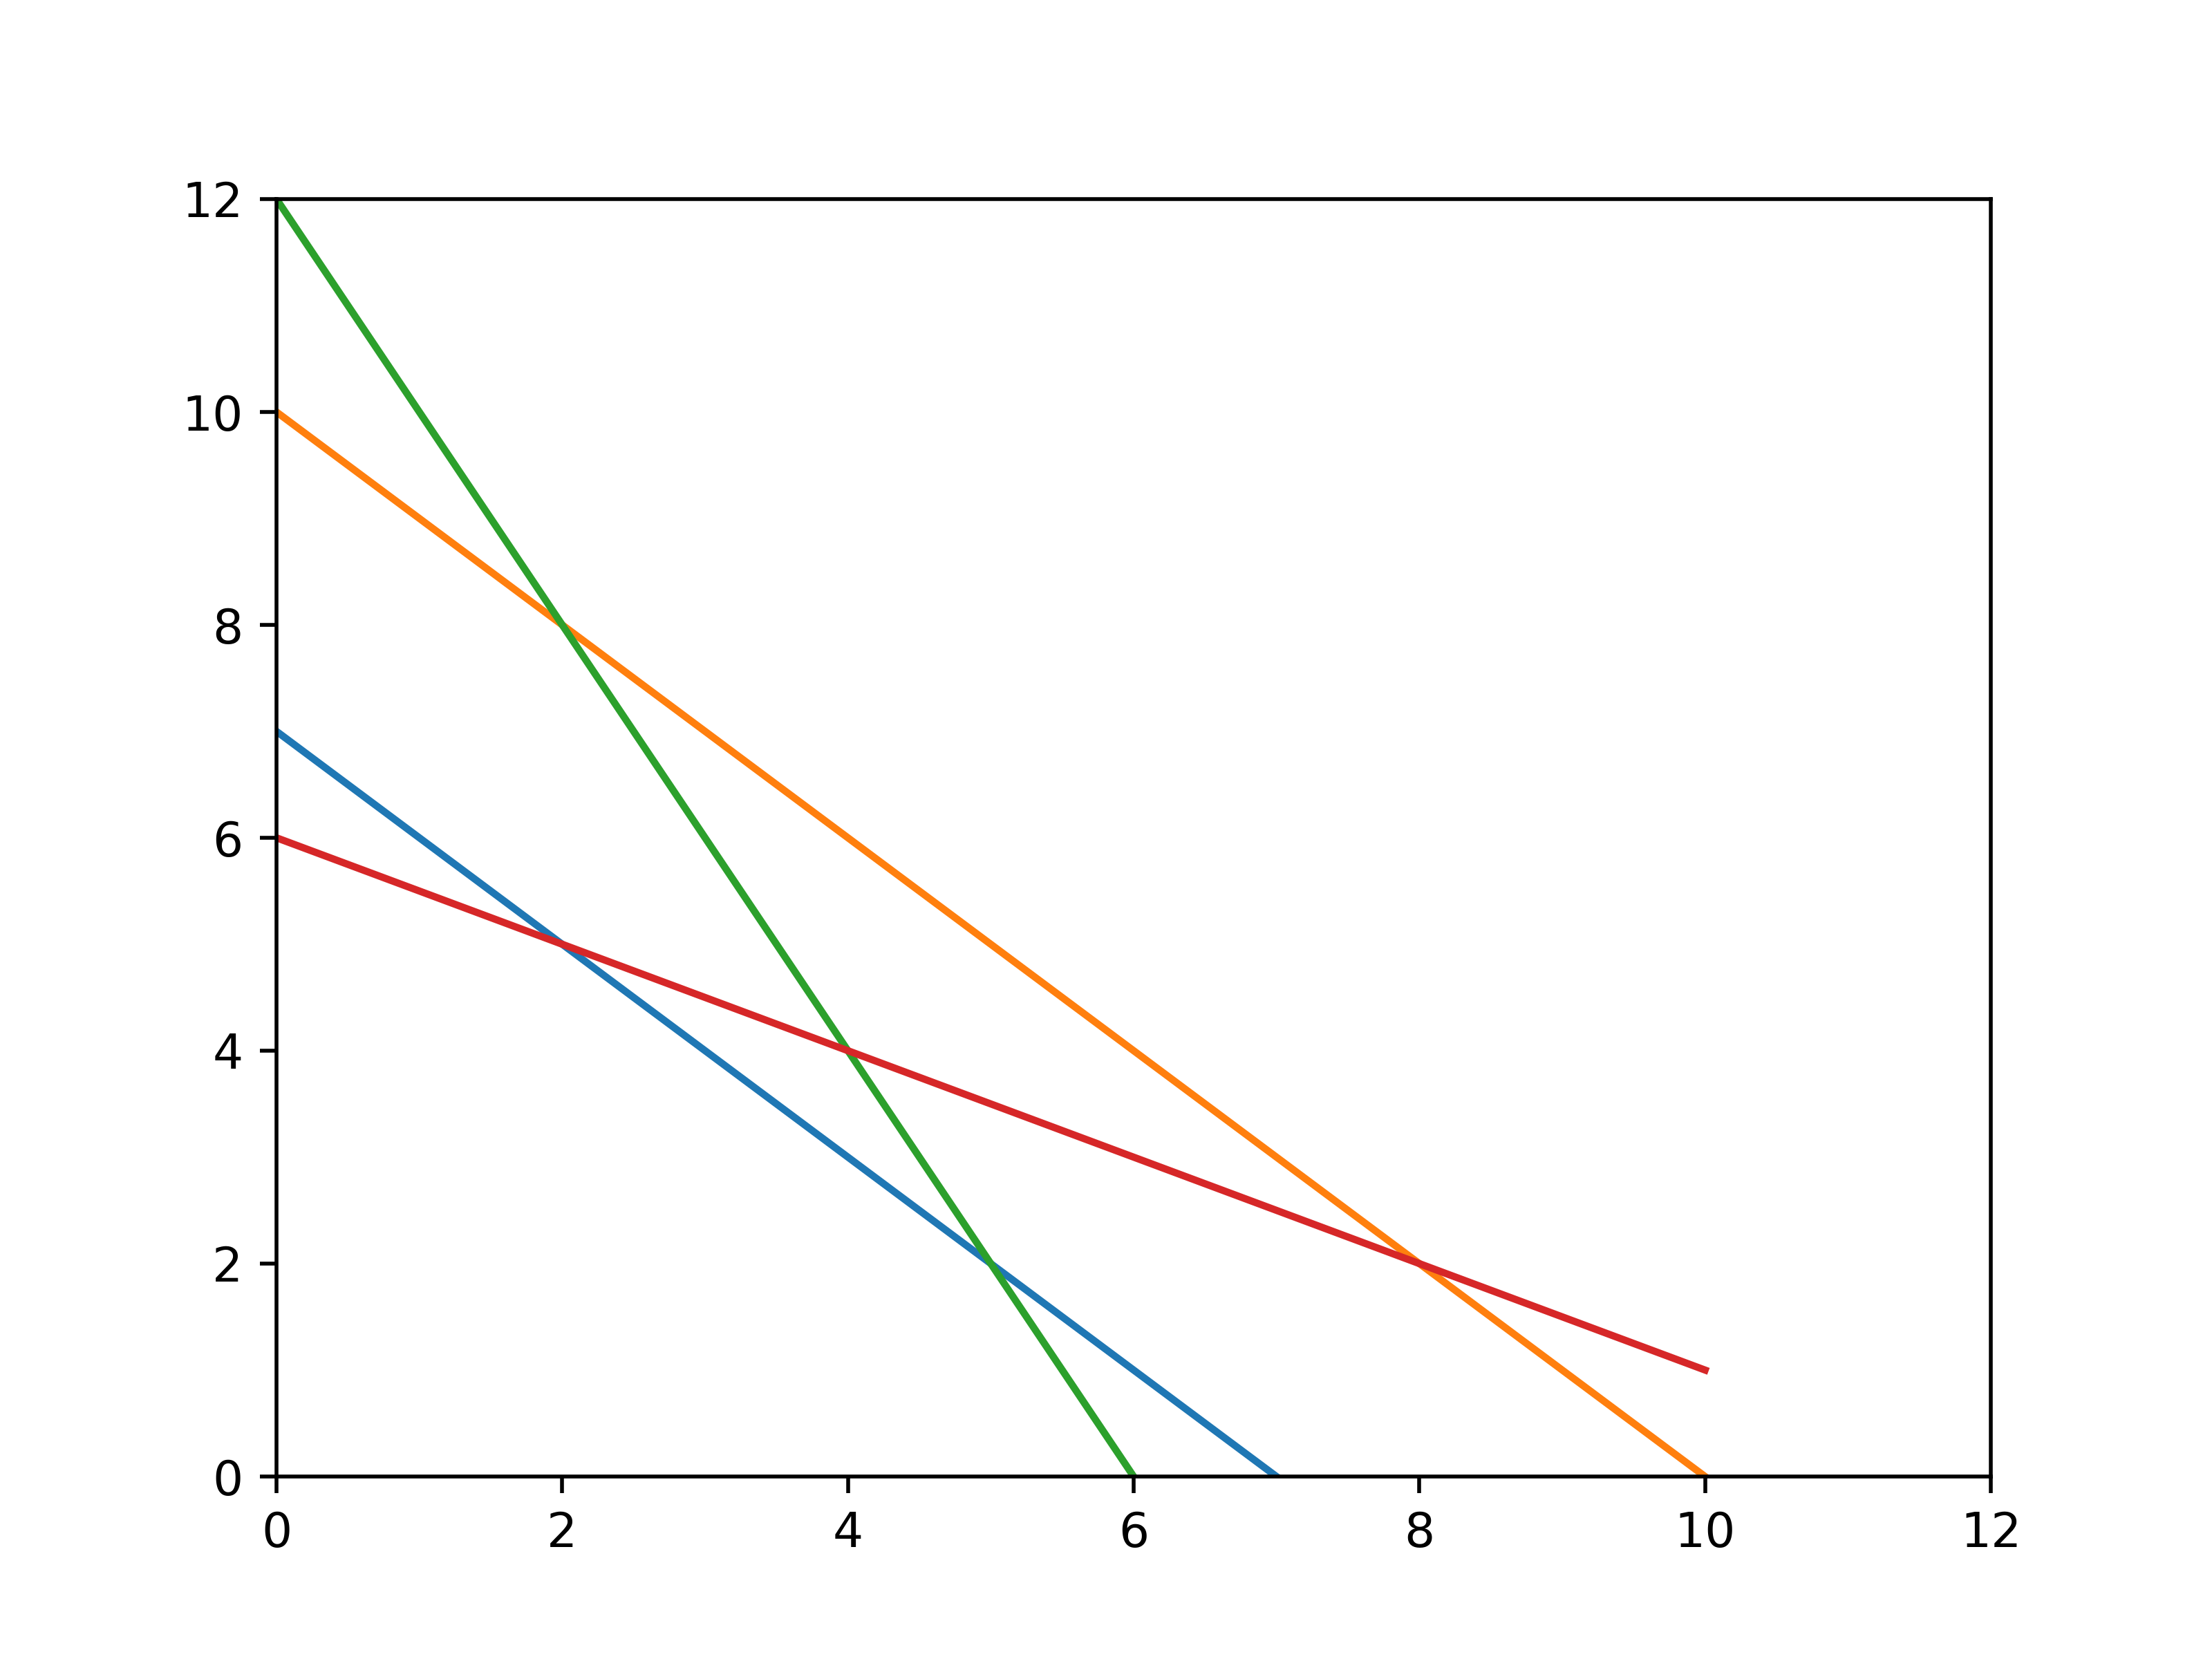
\includegraphics[width=.9\linewidth]{q5.png}
\end{center}
A região factível é o triângulo formado pelas restrições R1, R3 e R4.

Com isso, agora iremos achar os vértices desse triângulo, ou seja, os pontos
que são a intersecção de duas dessas 3 restrições:

\begin{itemize}
\item R1 com R3: \((5, 2)\)
\item R1 com R4: \((2, 5)\)
\item R3 com R4: \((4, 4)\)
\end{itemize}

Agora vamos avaliar o valor da função objetiva em cada um dos pontos:

\begin{itemize}
\item \(500*5+300*2 = 3100\)
\item \(500*2+300*5 = 2500\)
\item \(500*4+300*4 = 3200\)
\end{itemize}

A solução para o problema é o ponto \((4, 4)\), pois é o ponto que maximiza a função objetiva
satisfazendo as restrições. Ou seja, o fazendeiro deveria plantar 4 acres de cada.\newpage
\section{Questão 6}
\label{sec:orgb410b8c}
Formulando o problema temos 5 restrições:
\begin{itemize}
\item R1: \(a+b \geq 3\)
\item R2: \(2a+b \geq 8\)
\item R3: \(b \leq 2a\)
\item R4: \(a \geq 0\)
\item R5: \(b \geq 0\)
\end{itemize}

e queremos maximizar \(2a+3b\).

Aqui faremos a mesma coisa que no exercício anterior, vamos plotar e achar a região factível:

\begin{center}
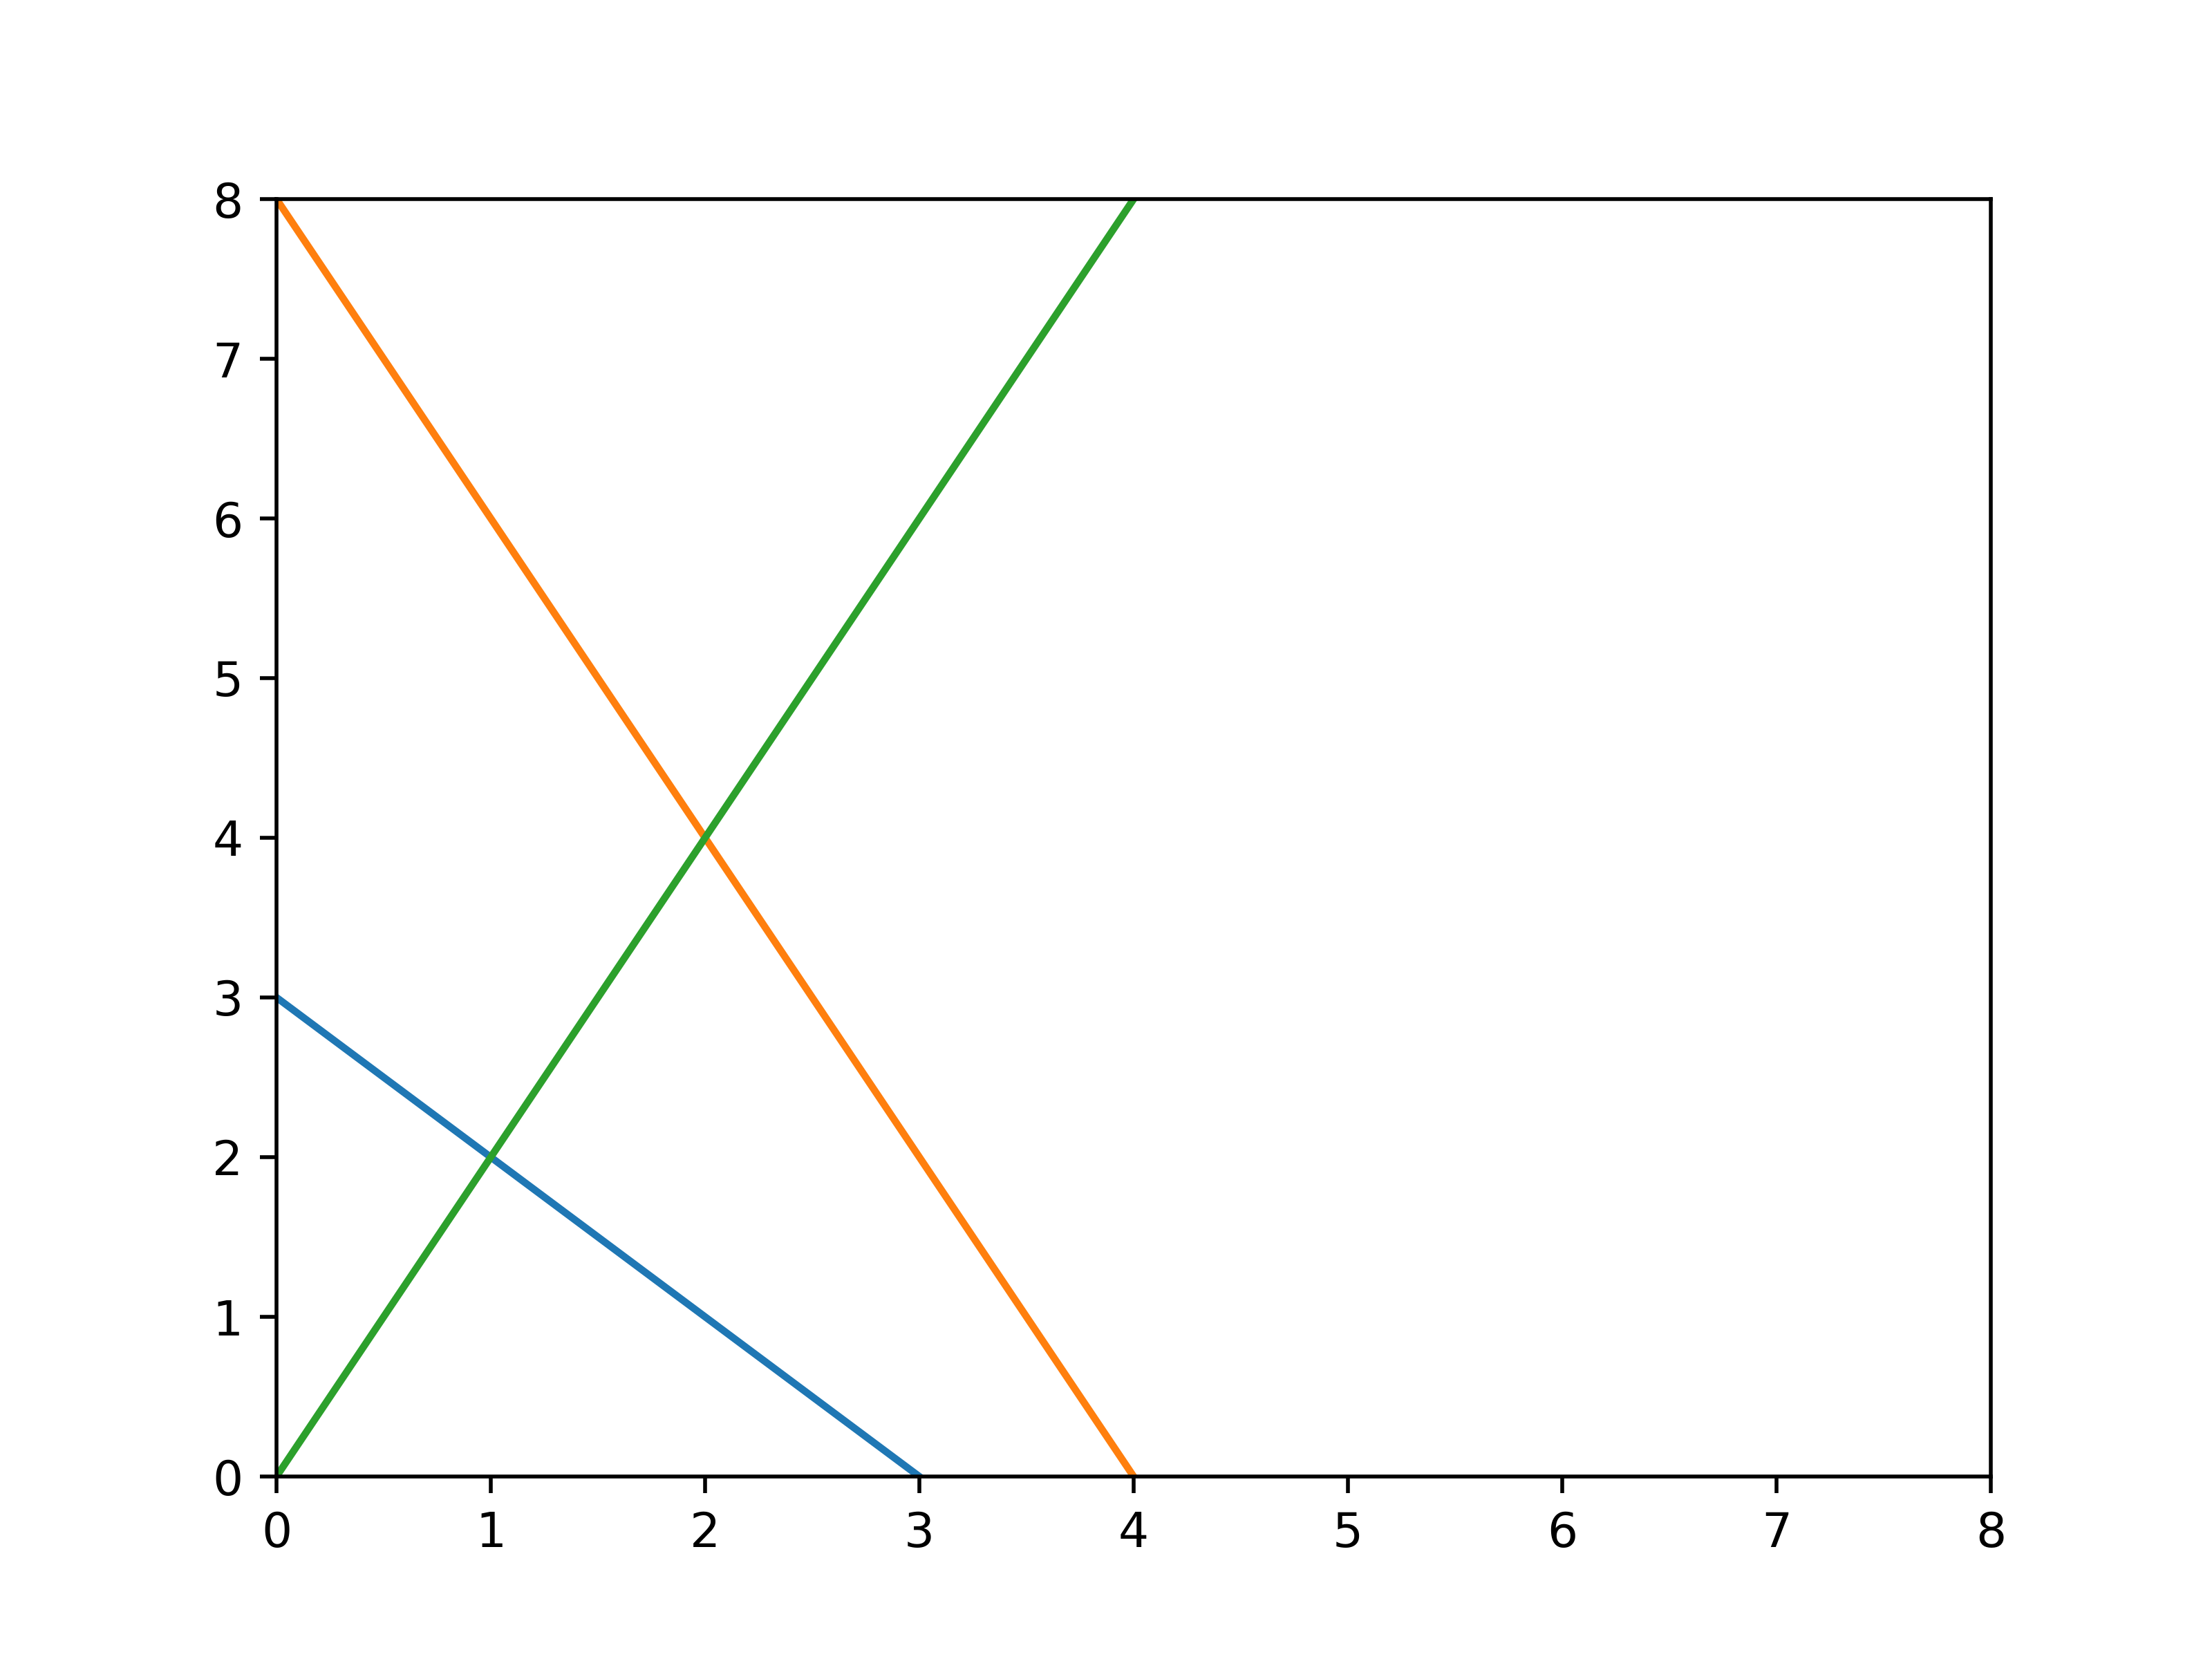
\includegraphics[width=.9\linewidth]{q6.png}
\end{center}

A região factível é o polígono formado pelas restrições R1, R2, R3 e R5.

Acharemos os vértices factíveis:
\begin{itemize}
\item R1 com R3: \((1, 2)\)
\item R1 com R5: \((3, 0)\)
\item R2 com R3: \((2, 4)\)
\item R3 com R5: \((4, 0)\)
\end{itemize}

Colocaremos os pontos na função objetiva e nossa solução será o que der o melhor resultado:
\begin{itemize}
\item \(2*1 + 3*2 = 8\)
\item \(2*3 + 3*0 = 6\)
\item \(2*2 + 3*4 = 16\)
\item \(2*4 + 3*0 = 8\)
\end{itemize}

Portanto nossa solução é o ponto \((2, 4)\), ou seja, processar 2 toneladas da fonte A e 4 da fonte B.
\section{Questão 7}
\label{sec:org1fd7f43}
\begin{itemize}
\item \(x_n\) é o número de livros enviados de Novato para São Francisco
\item \(y_n\) é o número de livros enviados de Novato para Sacramento
\item \(x_l\) é o número de livros enviados de Lodi para São Francisco
\item \(y_l\) é o número de livros enviados de Lodi para Sacramento
\end{itemize}

Formulando o problema temos 8 restrições:
\begin{itemize}
\item R1: \(x_n+x_l = 600\)
\item R2: \(y_n+y_l = 400\)
\item R3: \(x_n+y_n \leq 700\)
\item R4: \(x_l+y_l \leq 800\)
\item R5, R6, R7, R8: \(x_n,y_n,x_l,y_l \geq 0\)
\end{itemize}

e queremos minimizar \(5x_n+10y_n+15x_l+4y_l\).

Primeiro vamos expressar \(x_l\) e \(y_l\) em função de \(x_n\) e \(y_n\) para conseguirmos plotar as restrições.

\begin{itemize}
\item \(x_l = 600-x_n\)
\item \(y_l = 400-y_n\)
\end{itemize}

Isso nos dá um novo conjunto de restrições:
\begin{itemize}
\item R1: \(x_n+y_n \leq 700\)
\item R2: \(x_l+y_l = 600-x_n+400-y_n \leq 800 \rightarrow 200 \leq x_n+y_n\)
\item R3: \(x_n \geq 0\)
\item R4: \(y_n \geq 0\)
\item R5: \(x_l \geq 0 \rightarrow 600 \geq x_n\)
\item R6: \(y_l \geq 0 \rightarrow 400 \geq x_n\)
\end{itemize}

e a seguinte função objetiva: \(5x_n+10y_n+15(600-x_n)+4(400-y_n) = 10600 - 10x_n + 6y_n\)

Plotando e achando a região factível:

\begin{center}
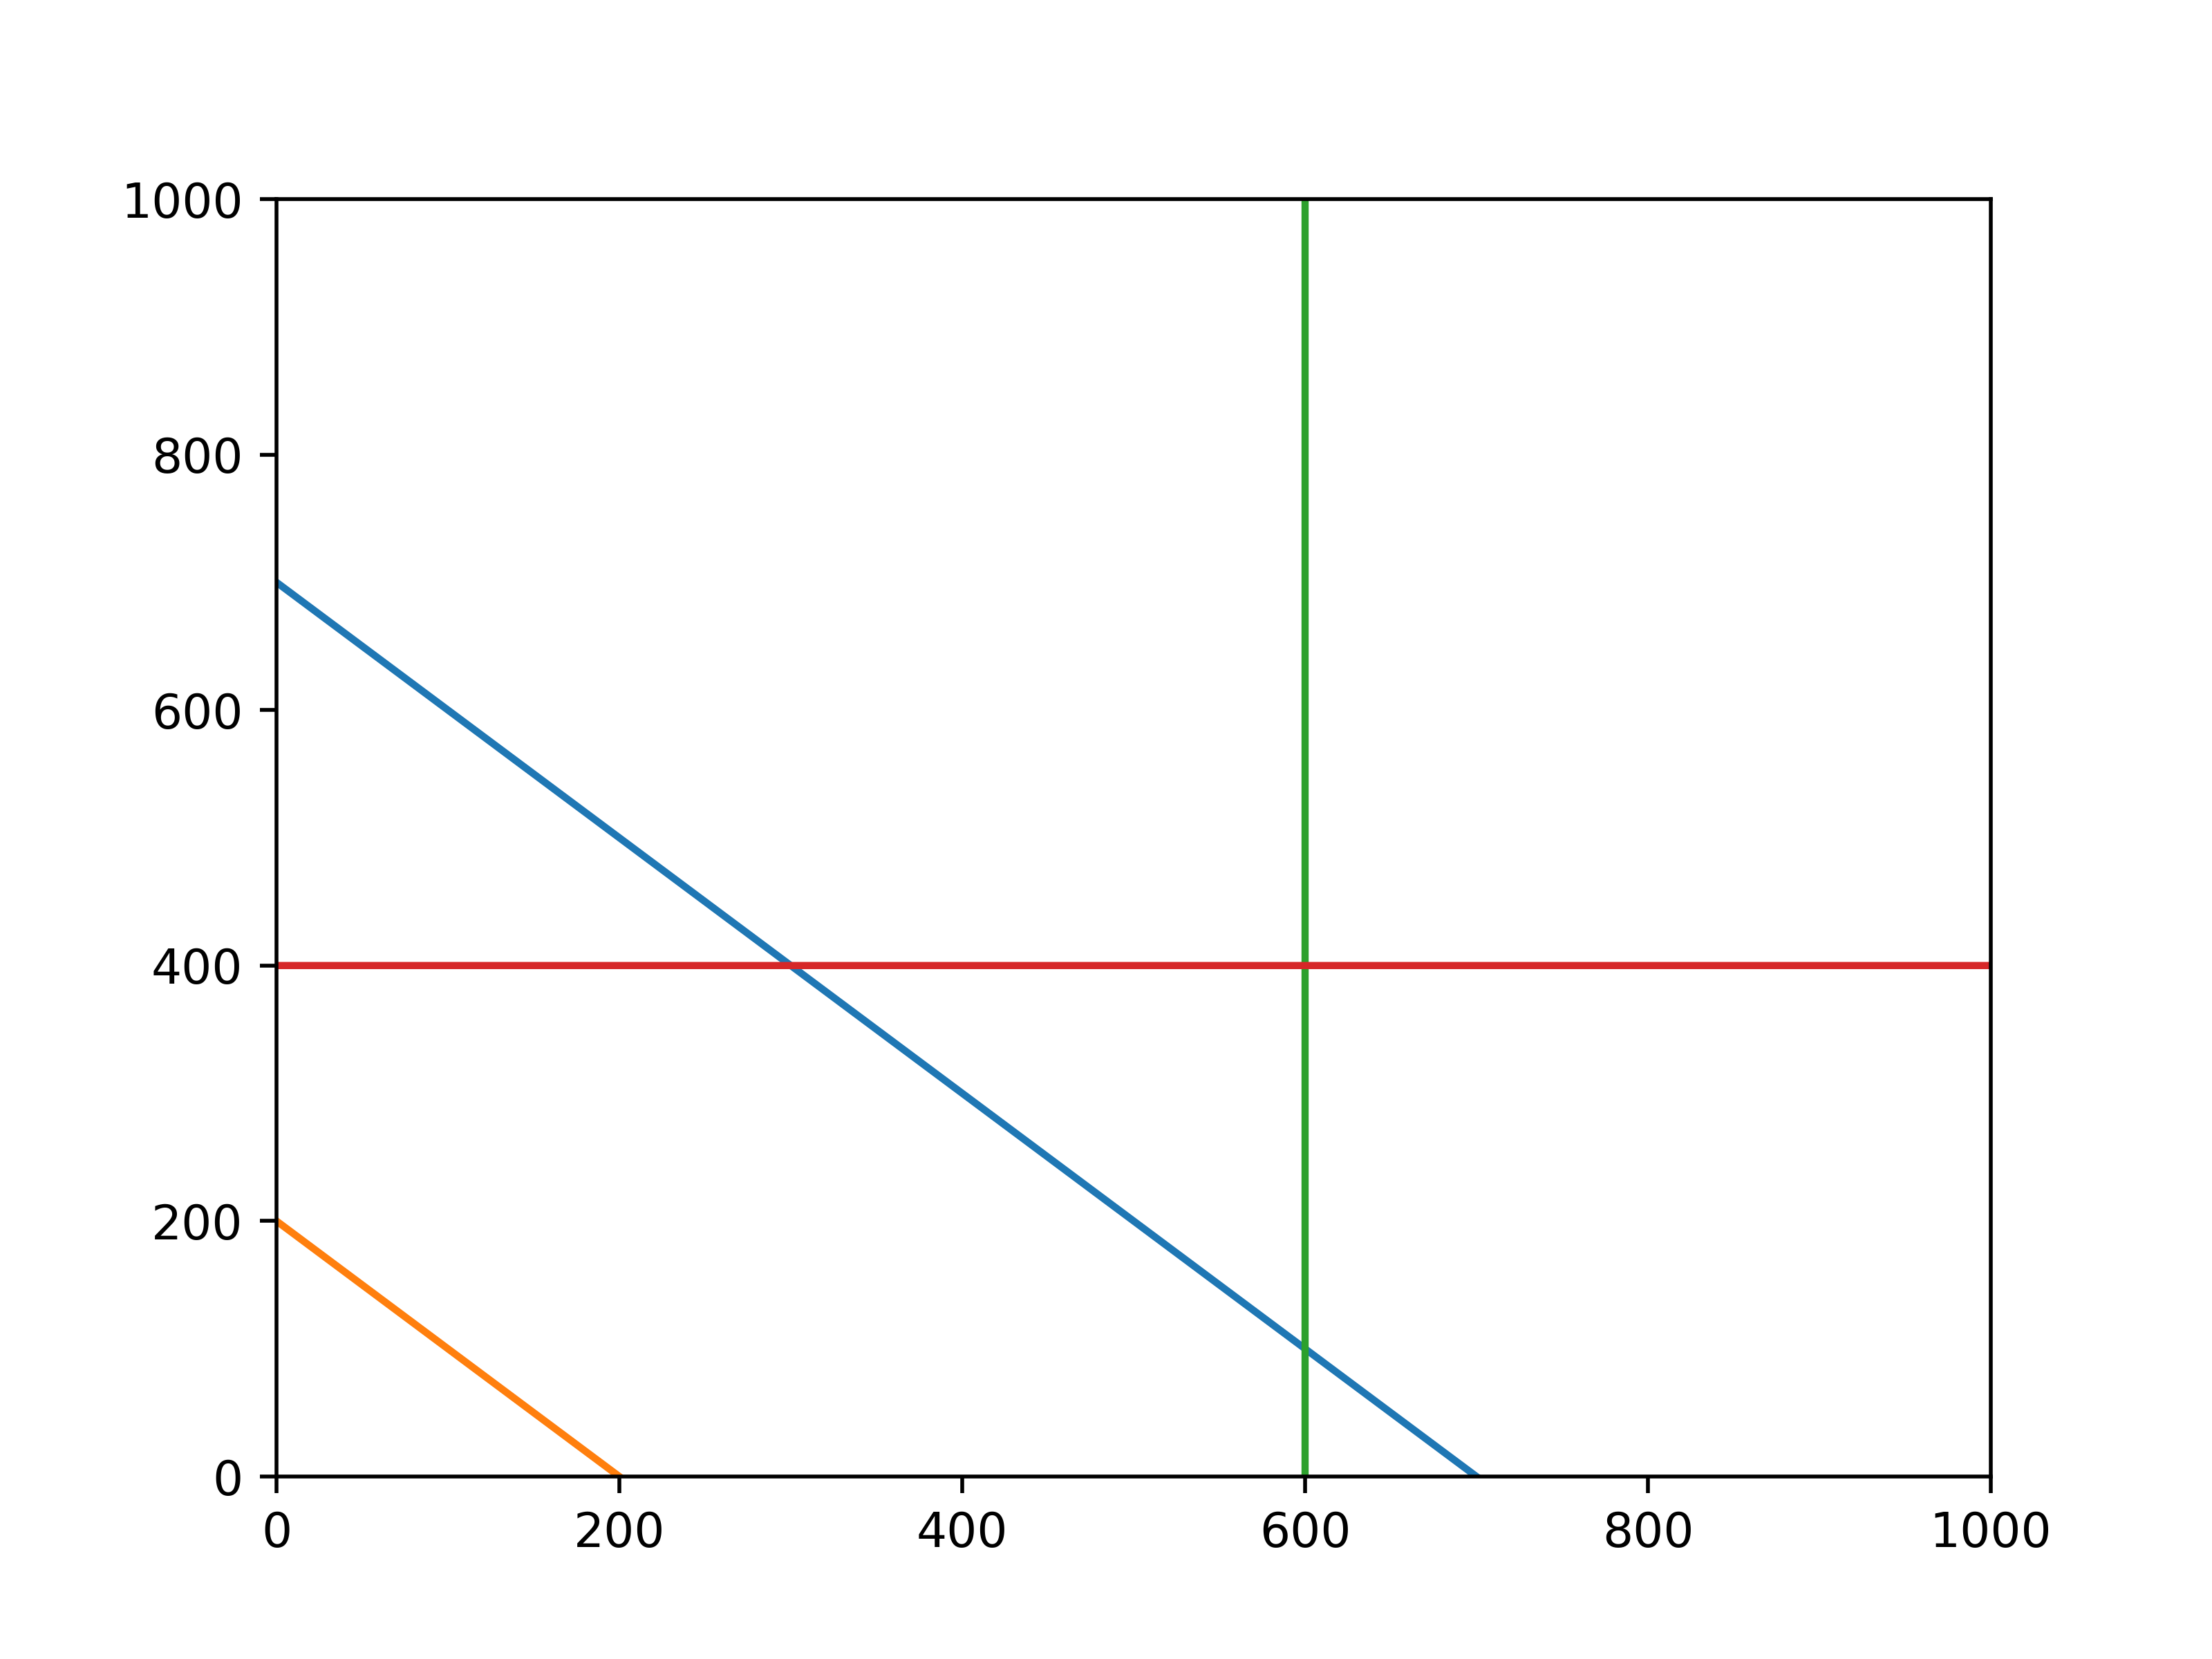
\includegraphics[width=.9\linewidth]{q7.png}
\end{center}

A região factível é o polígono formado pelas 6 restrições.

Acharemos os vértices factíveis:
\begin{itemize}
\item R1 com R5: \((600, 100)\)
\item R1 com R6: \((300, 400)\)
\item R2 com R3: \((0, 200)\)
\item R2 com R4: \((200, 0)\)
\item R3 com R6: \((0, 400)\)
\item R4 com R5: \((600, 0)\)
\end{itemize}

Colocaremos os pontos na função objetiva e nossa solução será o que der o melhor resultado:
\begin{itemize}
\item \(10600 - 10*600 + 6*100 = 5200\)
\item \(10600 - 10*300 + 6*400 = 10000\)
\item \(10600 - 10*0 + 6*200 = 11800\)
\item \(10600 - 10*200 + 6*0 = 8600\)
\item \(10600 - 10*0 + 6*400 = 13000\)
\item \(10600 - 10*600 + 6*0 = 4600\)
\end{itemize}


Portanto nossa solução é o ponto \((0, 400)\), ou seja, mandar 600 cópias de Novato pra São Francisco e mandar 400 de Lodi
para Sacramento.
\section{Questão 8}
\label{sec:orgaa6d782}
Primeiro vamos escrever o problema na forma canônica e vamos introduzir as varáveis novas:

\(\begin{cases}
  -2x+y+P = 0 \\
  2x+3y+s_1 = 3 \\
  x+5y+s_2 = 1 \\
  2x+y+s_3 = 4 \\
  4x+y+s_4 = 5 \\
  x,y \geq 0
  \end{cases}\)

Agora, vamos escrever na forma de matriz:

\begin{center}
\begin{tabular}{c c c c c c c | c}
x & y & s\textsubscript{1} & s\textsubscript{2} & s\textsubscript{3} & s\textsubscript{4} & P & RHS\\
2 & 3 & 1 & 0 & 0 & 0 & 0 & 3\\
1 & 5 & 0 & 1 & 0 & 0 & 0 & 1\\
2 & 1 & 0 & 0 & 1 & 0 & 0 & 4\\
4 & 1 & 0 & 0 & 0 & 1 & 0 & 5\\
\hline
-2 & -1 & 0 & 0 & 0 & 0 & 1 & 0\\
\end{tabular}
\end{center}

Escolherei o x como pivô, e usarei a linha 2 para o processo de trocar a base:

\begin{center}
\begin{tabular}{c c c c c c c | c}
x & y & s\textsubscript{1} & s\textsubscript{2} & s\textsubscript{3} & s\textsubscript{4} & P & RHS\\
0 & -7 & 1 & -2 & 0 & 0 & 0 & 1\\
1 & 5 & 0 & 1 & 0 & 0 & 0 & 1\\
0 & -9 & 0 & -2 & 1 & 0 & 0 & 2\\
0 & -19 & 0 & -2 & 0 & 1 & 0 & 1\\
\hline
0 & 9 & 0 & 2 & 0 & 0 & 1 & 2\\
\end{tabular}
\end{center}

O que fiz para zerar a primeira coluna com exceção da segundalinha foi:

\begin{itemize}
\item Subtrai \(2L_2\) de \(L_1\)
\item Subtrai \(2L_2\) de \(L_3\)
\item Subtrai \(4L_2\) de \(L_4\)
\item Adcionei \(2L_2\) em \(L_5\)
\end{itemize}

Todos os valores da última linha agora são positivos, indicando que achamos a solução. Nossas variáveis livres são
\(y\) e \(s_2\), ou seja, trocaremos elas por 0 na nossa solução. Com o sistemas de equação que temos e trocando \(x\) e
\(s_2\) por 0, temos que:

\begin{itemize}
\item \(x=1\)
\item \(y=0\)
\item \(s_1=1\)
\item \(s_2=0\)
\item \(s_3=2\)
\item \(s_4=1\)
\end{itemize}

Ou seja, o valor máximo é 2, que ocorre quando \(x\) é 1 e \(y\) é 0.
\section{Questão 9}
\label{sec:org223bbfc}
\begin{itemize}
\item Se \(a\) ou \(b\) são 0, o problema não tem solução, pois o gradiente invertido irá apontar pra uma direção que sempre podemos
ir, ou seja, podemos deixar o custo infinitamente menor.
\item Se \(a = 0\) e \(b = 0\), qualquer ponto dentro da região factível é um ponto ótimo pois nosso gradiente será \((0, 0)\) sempre.
\item Se \(a = 0\) e \(b > 0\), qualquer ponto tal que \(y = 0\) e \(x \geq 6\) é ótimo. Isso acontece pois se o \(x\) for maior ou igual à 6 nós estaremos dentro da região factível e o nosso gradiente é perpendicular ao eixo x, ou seja, nossa solução se encontra nessa reta.
\item Se \(a > 0\) e \(b = 0\), o argumento de cima vale para o eixo y ao invés do x.
\item Se o vetor \((a, b)\) for paralelo ao vetor \((2, 1)\), toda a reta \(2x+y = 6\) será uma solução ótima, desde que o ponto escolhido esteja dentro da região factível
\item Se o vetor \((a, b)\) for paralelo ao vetor \((1, 2)\), toda a reta \(x+2y = 6\) será uma solução ótima, desde que o ponto escolhido esteja dentro da região factível
\item Por último, se \(a, b > 0\) temos 3 subcasos:
\begin{itemize}
\item Se \((a, b)\) pode ser escrito como \(\alpha(1, 0)+\beta(2, 1)\) com \(\alpha,\beta>0\) temos que a solução ótima será o ponto \((0, 6)\).
\item Se \((a, b)\) pode ser escrito como \(\alpha(2, 1)+\beta(1, 2)\) com \(\alpha,\beta>0\) temos que a solução ótima será o ponto \((2, 2)\).
\item Se \((a, b)\) pode ser escrito como \(\alpha(0, 1)+\beta(1, 2)\) com \(\alpha,\beta>0\) temos que a solução ótima será o ponto \((6, 0)\).
\end{itemize}
\end{itemize}

\section{Questão 10}
\label{sec:org2bb2211}
\begin{itemize}
\item Se \(a\) e \(b\) são 0, todos os pontos da região factível são ótimos.
\item Se \(b < 0\) ou se \(a > 0\), não temos solução ótima.
\item Se \(b = 0\) e \(a < 0\), a reta \(x = 4\) é solução ótima desde que \(y \geq 6\)
\item Se \(a = 0\) e \(b > 0\), a reta \(y = 0\) é solução ótima desde que \(x \leq -2\)
\item Se o vetor \((a, b)\) for paralelo ao vetor (-2, 1), toda a reta \(-2x+y \geq -2\) é solução ótima, desde que o ponto escolhido esteja dentro da região factível
\item Se o vetor \((a, b)\) for paralelo ao vetor (-1, 2), toda a reta \(-x+2y \geq 2\) é solução ótima, desde que o ponto escolhido esteja dentro da região factível
\item Por último, se \(a < 0\) e \(b > 0\), temos 3 subcasos:
\begin{itemize}
\item Se \((a, b)\) pode ser escrito como \(\alpha(-2, 1)+\beta(-1, 0)\) com \(\alpha,\beta>0\) temos que a solução ótima será o ponto \((4, 6)\).
\item Se \((a, b)\) pode ser escrito como \(\alpha(-2, 1)+\beta(-1, 2)\) com \(\alpha,\beta>0\) temos que a solução ótima será o ponto \((2, 2)\).
\item Se \((a, b)\) pode ser escrito como \(\alpha(-1, 2)+\beta(0, 1)\) com \(\alpha,\beta>0\) temos que a solução ótima será o ponto \((-2, 0)\).
\end{itemize}
\end{itemize}
\end{document}